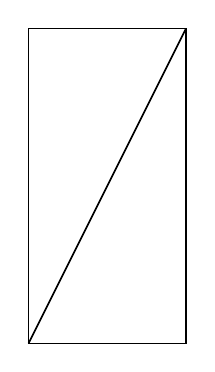
\begin{tikzpicture}[x=1cm,y=1cm,font=\normalsize,
 geometry edge/.style={solid,line width=.6pt},
 geometry mark/.style={solid,line width=.6pt},
 geometry label/.style={font=\normalsize,inner sep=2pt}]
\coordinate (Q1) at (0,0);
\coordinate (Q2) at (2,0);
\coordinate (Q3) at (2,4);
\coordinate (Q4) at (0,4);
\draw[geometry edge] (Q1)--(Q2)--(Q3)--(Q4)--cycle;
\draw[geometry edge] (Q1)--(Q3);
\end{tikzpicture}
